\documentclass[a4paper, twocolumn]{article}
\usepackage[pdftex]{graphicx}                % Improved inclusion of .pdf-graphics files.
\usepackage{sidecap}                         % Floats with captions to the right/left.
\usepackage{enumerate}                       % Change counters (arabic, roman, etc.).
\usepackage{floatrow}                        % Multi-figure floats.
\usepackage{subfig}                          % Multi-figure floats.
\usepackage{bm}                              % Bolded text in math mode.
\usepackage[framemethod=default]{mdframed}   % Make boxes.
\usepackage{listings}                        % For including source code.
\usepackage{mathtools}                       % Underbrackets, overbrackets.
\usepackage[dvipsnames]{xcolor}              % Colors.
\usepackage{capt-of}                         % Caption things which are not floats.
\usepackage{fontawesome}                     % Github icon, etc. \faGithub
\usepackage{sidecap}                         % Floats with captions on the side.
\usepackage{tabularx}                        % Tables and stuff.
\usepackage{tabulary}                        % Tables and stuff.
\usepackage[sf,sl,outermarks]{titlesec}      % Change fonts in section{}, subsection{}, etc.
\usepackage[subfigure]{tocloft}              % Change spacing between numbers and titles in TOC.
\usepackage{booktabs}                        % \toprule, \midrule, etc. for tables.
\usepackage{siunitx}                         % Allows S table column, aligning on decimal point.
\usepackage{chngcntr}                        % Change counter behaviour, supress increment of sub counters.
\usepackage[%                                % Adds functionality to captions.
tableposition = top,
labelsep      = period,
justification = raggedright,
format        = hang,
]{caption}
\usepackage[%                                % Interactive references and links, colored.
colorlinks  = true,
linkcolor   = black,
urlcolor    = blue,
citecolor   = black,
linktocpage = true,
]{hyperref}
\usepackage[%                                % References, in super-script form.
autocite    = superscript,
backend     = biber,
sortcites   = true,
style       = numeric-comp,
sorting     = none,
url         = false,
]{biblatex}
%

\newcommand{\x}{\bm{x}}
\newcommand{\C}{\mathbb{C}}
\newcommand{\X}{\bm{X}}
\newcommand{\diag}[1]{\mathrm{diag}(#1)}
\newcommand{\MSE}[1]{\mathrm{MSE}(#1)}
\newcommand{\R}[1]{\mathrm{R}^2(#1)}
\newcommand{\expect}{\mathbb{E}}
\newcommand{\var}{\mathbb{V}}
\newcommand{\cov}{\mathrm{Cov}}
\newcommand{\OLS}{\mathrm{OLS}}
\newcommand{\SD}{\mathrm{SD}}
\newcommand{\ridge}{\mathrm{ridge}}
\newcommand{\lasso}{\mathrm{lasso}}
\newcommand{\python}{\textsf{Python}{}}
\newcommand{\sgn}{\,\mathrm{sign}{}}

\newcommand{\mat}[1]{\bm{#1}}
\newcommand{\y}{\bm{y}}
\newcommand{\data}{\bm{\Omega}}
\newcommand{\cost}{\mathcal{C}}
\newcommand{\N}{\mathcal{N}}
\newcommand{\basis}{\mathcal{B}}
\usepackage{biblatex}
\usepackage[autostyle, english = american]{csquotes} % Assure quotation marks are inserted correctly aligned left/right.
\MakeOuterQuote{"}

% Package settings ----------------------------------------------------------- %
%\renewcommand{\thesection}{\Roman{section}}         % I, II, III, IV, etc. section numbering
%\renewcommand{\thesubsection}{\Alph{subsection}}    % A, B, C, etc. subsection numbering
\renewcommand{\thesubsubsection}{}                  % Remove subsubsection numbering.
\floatsetup[table]{capposition=top}                 % Place table captions above the table.
\captionsetup[subfigure]{labelformat=empty}         % Remove the (a), (b), etc. tags from subfigures.
\advance\cftsecnumwidth 1.0em\relax                 % Set the spacing between section headings and titles in TOC with tocloft.
\advance\cftsubsecindent 1.0em\relax                % Set the spacing between subsection headings and titles in TOC with tocloft.
\advance\cftsubsecnumwidth 1.0em\relax              % Set the spacing between subsubsection headings and titles in TOC with tocloft.
\newcommand{\listingsfont}{\ttfamily}
\newcommand{\inlinepy}[1]{\lstinline[language={python}]{#1}}
\newcommand{\inlinecc}[1]{\lstinline[language={c++}]{#1}}
\counterwithout*{subsection}{section}               % Dont reset the subsection counter on new \section{} calls.
\renewcommand{\figurename}{FIG.}                    % Captions of figures read FIG.
\renewcommand{\tablename}{TABLE}                    % Captions of tables read TABLE
\renewcommand{\thetable}{\Roman{table}}             % Number tables with roman numerals.

% Section headings settings -------------------------------------------------- %
\titleformat{\section}[hang]  % {command}[shape]
{\normalfont\bfseries}      % {format}
{\thesection.}              % {label}
{2ex}                       % {sep}
{\centering\MakeUppercase}  % {before-code}[after-code]

\titleformat{\subsection}[hang] % {command}[shape]
{\normalfont\bfseries}        % {format}
{\thesubsection.}             % {label}
{1ex}                         % {sep}
{\centering}                  % {before-code}[after-code]

\titleformat{\subsubsection}[hang]  % {command}[shape]
{\normalfont\bfseries}            % {format}
{}                                % {label}
{1ex}                             % {sep}
{\centering}                      % {before-code}[after-code]


% References ----------------------------------------------------------------- %
\newcommand{\Fig}[1]{Fig.\ \ref{fig:#1}}
\newcommand{\fig}[1]{Fig.\ \ref{fig:#1}}
\newcommand{\eq} [1]{Eq.\ (\ref{eq:#1})}
\newcommand{\Eq} [1]{Eq.\ (\ref{eq:#1})}
\newcommand{\tab}[1]{Table \ref{tab:#1}}
\newcommand{\Tab}[1]{Table \ref{tab:#1}}


% Manually set alignment of rows / columns in matrices (mat, pmat, etc.) ----- %
\makeatletter
\renewcommand*\env@matrix[1][*\c@MaxMatrixCols c]{%
  \hskip -\arraycolsep
  \let\@ifnextchar\new@ifnextchar
  \array{#1}}
\makeatother

% figures in multicols environment ------------------------------------------- %
\newenvironment{Figure}
{\par\medskip\noindent\minipage{\linewidth}}
{\endminipage\par\medskip}

% Set bibliography file and path for images.
\addbibresource{ref.bib}
\bibliography{ref.bib}
\graphicspath{{../figs/}}

% Black frame with gray background ------------------------------------------ %
\definecolor{gray}{gray}{0.9}
\newmdenv[linecolor=white,backgroundcolor=gray]{grayframe}

% Title
\title{{\sc Regression and Resampling methods \\ {\large FYS-STK4155: Project 1}}}
\author{Trygve Leithe Svalheim \\ \faGithub \ {\small \href{https://github.com/trygvels/FYS-STK4155}{github.com/trygvels/FYS-STK4155}}}
  

\begin{document}


\twocolumn[
\begin{@twocolumnfalse}
\maketitle
\begin{abstract}
We look at three different types of regression methods and their ability to fit a polynomial of varying degree to two different types of data. We look at Ordinary Least Squares (OLS), Ridge and Lasso regression and discuss their advantages and hyper parameters. Additionally, we discuss the advantages of resampling methods and the bias-variance trade-off problem. We conclude that OLS is the better method for fitting to the mathematically produced and predictable Franke function data, but that we obtain the lowest error for the terrain data using a regularizing term with Ridge regression.
\end{abstract}

\tableofcontents 
\end{@twocolumnfalse}]
\clearpage
%\newpage
%% INTRODUCTION
\section{Introduction}

In this project we explore the problem of regression analysis, resampling and optimal hyperparemeters. Regression is the process modelling a response $\tilde{y}$ to true observed data $y$ from a predictor variable $x$ to learn about the relationship between data. In this work, our focus will be on Linear regression, where the relationship between $x$ and $y$ is strictly linear and can be described by the model
\begin{equation}
  \mathbf{\tilde{y}} = \mathbf{X}\mathbf{\beta},
\end{equation}
and the true response can be described with the addition of an error term $\epsilon$, denoting the modelling error so that
\begin{equation}
  \mathbf{y} = \mathbf{X}\mathbf{\beta}+\mathbf{\epsilon}.
\end{equation}
Linear regression is a fundamental method of statistical analysis, and allows us to study the relationships hidden in all types of data sets, which is increasingly powerful in a world where data is both abundant and complex.
In this study, we look at three common regression methods and assess their capabilities on two different data sets. In addition, we explore the importance resampling methods and the impact of hyper-paremeters and their data dependence.

%% -----------------
\section{Regression methods}
In this section we outline the basics of three different regression methods which we later apply to our two data sets. If not otherwise stated, we are following the course lecture notes\autocite{MHJ}. 
\subsection{Ordinary Least Squares (OLS)}
As briefly mentioned in the introduction, a Linear regression system revolves around modeling a function $\mathbf{y}(\mathbf{X})$, where the matrix $\mathbf{X}$ containing the predictors is called \textit{design matrix}. Again, we want to find the values of $\beta$, that minimizes the error $\epsilon$ describing the difference between the predicted and true values $\mathbf{\tilde{y}}$ and $\mathbf{y}$.
However, there are several different ways of describing the error, for the first method, the \textit{Ordinary Least Squares (OLS)} method, we chose a \textit{cost function} parameterized by the Euclidean $L^2$ norm,
\begin{align}
C(\bm\beta) &= \Vert \mathbf{y} - \tilde{\mathbf{y}}\Vert_2^2 \nonumber \\
&= \sum_{i=1}^n \Big| y_i - \sum_{j=0}^p X_{ip} \beta_p \Big|^2. \label{eq:cost}
\end{align}
Furthermore we can quantize the full error using the \textit{Mean Squared Error} (MSE), which is simply the ensamble average over the $L^2$-loss. 
For this particular error metric, the optimal $\beta$ parameters can be found by minimising this function.
The linear algebra representation of this minimization problem can be described following Hastie, Tibshirani \& Friedman\autocite{trevor2009elements} by

\begin{align}
\frac{\partial C(\bm\beta)}{\partial \bm\beta} &= \frac{\partial}{\partial \bm\beta} (\mathbf{y}-\mathbf{X}\bm\beta)^T (\mathbf{y}-\mathbf{X}\bm\beta) = 0 \nonumber \\
\bm\beta_\text{optimal} &= \left(\mathbf{X}^T\mathbf{X}\right)^{-1}\mathbf{X}^T\mathbf{y}.
\end{align}
For some datasets, the inversion operation $\left(\mathbf{X}^T\mathbf{X}\right)$ is too costly. With the data sizes we are dealing with this should not lead to any problems. However, in order to generalize our program, we chose to employ the Singular Value Decomposition (SVD) method. Without going into the nits and grits of the derivation of the method, we decompose the matrix $X$ into more computationally tractable matrices;
\begin{align}
\mathbf{X} = \mathbf{U}\mathbf{\Sigma}\mathbf{V}^T.
\end{align}
Using this definition, it can be shown that
\begin{align}
\tilde{\mathbf{y}}_\text{OLS} &= \mathbf{X}\bm\beta_\text{OLS} \nonumber \\
&= \mathbf{X}\left(\mathbf{X}^T\mathbf{X}\right)^{-1}\mathbf{X}^T\mathbf{y} \nonumber \\
&= \mathbf{X} \left[ \left(\mathbf{U}\bm\Sigma \mathbf{V}^T\right)^T \mathbf{U}\bm\Sigma \mathbf{V}^T \right]^{-1} \mathbf{X}^T \mathbf{y} \nonumber \\
&= \mathbf{U}\mathbf{U}^T\mathbf{y}. \label{eq:principal1}
\end{align}
The OLS method is thus a simple and straight forward method which is surprisingly powerful even without a regularization term, which is the key difference between it and Ridge regression.

\subsection{Ridge regression}
A common problem in regression and machine learning is over-fitting. When the complexity of the model increases, the system tries too hard to fit the training data, ultimately increasing the error on the test data. Ridge regression attempts to combat this by introducing an alternative cost function
\begin{align}
  C(\boldsymbol{X},\boldsymbol{\beta})=\frac{1}{n}\vert\vert \boldsymbol{y}-\boldsymbol{X}\boldsymbol{\beta}\vert\vert_2^2+\lambda\vert\vert \boldsymbol{\beta}\vert\vert_2^2.
\end{align}
With the addition of a regularization term, quantified by the hyper-parameter $\lambda$, we penalize high values of $\beta$. This effectively simplifies the solution, making the model less flexible, reducing the variance. The drawback, however, is that this also increases the bias if the \textit{shrinkage parameter} $\lambda$ is not chosen optimally. As we will later discuss, when increasing the complexity of our model, our system becomes increasingly susceptible to over-fitting the training data. With the implementation of the regularization term, we force the system to converge on a ``simple'' model, effectively reducing the variance. 

\subsection{Lasso regression}
The last of the trio is Lasso regression. It is similar to Ridge in the way that it adds a regularization term, but more aggressively so. This becomes evident when we once again look at the cost function
\begin{align}
  C(\boldsymbol{X},\boldsymbol{\beta})=\frac{1}{n}\vert\vert \boldsymbol{y}-\boldsymbol{X}\boldsymbol{\beta}\vert\vert_2^2+\lambda\vert\vert \boldsymbol{\beta}\vert\vert_1.
\end{align}
Here, the regularization comes on the form of $L^1$, which forces $\beta$-values to zero for sufficiently large values of $\lambda$. This creates a sparse $\beta$-array, as only certain polynimials (in our case) are activated, as opposed to Ridge regression, where high-degree polynomials with very low $\beta$-values are still present.

\section{Data}
In this project we have tested the three previously discussed regression methods on two different data sets. First, we fit a polynomial to the \textit{Franke function}, a common test function for such analyses. Last, we assess our polynomial regression fits on real world terrain data. In both cases the data is split into a training data set and a test data set, more on this in the next section.
\subsection{The Franke Function}
The Franke function is a two dimensional function developed to test interpolation techniques. However, its geometric features are well suited for our surface regression analysis as well \autocite{franke}. Mathematically, the Franke function is expressed as
\begin{align}
f_\text{F}(x,y) &= \frac{3}{4}\exp\left\{\frac{-1}{4}\left[\left(9x-2\right)^2 + \left(9y-2\right)^2\right]\right\}\nonumber \\
&+ \frac{3}{4}\exp\left\{\frac{-1}{49}\left(9x+1\right)^2 + \frac{1}{10}\left(9y+1\right)^2\right\}\nonumber \\
&+ \frac{1}{2}\exp\left\{\frac{-1}{4}\left[\left(9x-7\right)^2 + \left(9y-3\right)^2\right]\right\}\nonumber \\
&- \frac{1}{5}\exp\left\{\frac{-1}{4}\left[\left(9x+4\right)^2 + \left(9y-7\right)^2\right]\right\}.
\end{align}
A surface plot of the Franke function can be seen in figure \ref{fig:OLSfranke} evaluated over $x,y \in [0,1]$. 

\subsection{Terrain data}
The other data set employed in this study is taken from the U.S. Department of the Interior Geological Surveys (USGS) EarthExplorer website. The data is gathered from a Shuttle Radar Topography Mission (SRTM), an instrument on board the space shuttle Endeavor, which used radar interferometry to map out terrain. More specifically, the area of land we are using is that of M\o svatn in Telemark visualized in figure \ref{fig:terrain}. In our analysis, we have chosen to down-sample it by averaging to a $60\times 30$ matrix grid, which hopefully still carries distinctly different geometrical properties to that of the Franke function.

\section{Resampling and Bias variance}
Making predictions can be hard, and even harder with insufficient data. Therefore, effective resampling methods are vital to modern statistics. Resampling is the process of refitting the model to different samples of ones data set. By doing this, we can obtain additional information about our model fits than we would from fitting just once as we can learn something about how our fit varies within our data set. One drawback to this, however, is computational expense, which again, for our study is not an issue.

As previously stated, we split our data set randomly into two main sets; the training data containing $80 \%$ of all data and the test data, the remaining $20\%$. In order to make sure these are representable samples of our data set, as well as studying the variance in our predictions, we apply what is called \textit{K-Fold Cross-validation}, which splits the data into $k$ number of equally sized but mutually exclusive subsets, meaning that when one set is used as test data, the rest of the data is used for training. Once the model is fit to one of the k-fold test data sets, another one of the subsets are chosen, and the rest are again used as training data, So that in the end, all subsets have been used as test data once.

This method allows us to study the variance of the $\beta$ coefficients, and calculate a confidence interval, which is useful in determining the reliability of our model. Furthermore, we test our model fit using a Mean Squared Error (MSE), as defined in our discussion of OLS. We also calculate the coefficient of determination $R^2$ which is closely related to the MSE, we will focus on MSE for our study.  During model assessment and selection; determining the optimal flexibility of our model, we study how the error behaves. This is where the \textit{Bias-Variance tradeoff} comes in. In order to determine the optimal hyper-parameters and model complexity for our system, we need to look at how the MSE responds as a function of model complexity. By decomposing the MSE as 
\begin{align}
    \mathbb{E}&\left[(\boldsymbol{y}-\boldsymbol{\tilde{y}})^2\right]=    \mathbb{E}\left[(\boldsymbol{y}+\boldsymbol{f}-\boldsymbol{f}-\boldsymbol{\tilde{y}})^2\right]\\ 
    =& \frac{1}{n}\sum_{i=1}^n\left\{\overbrace{\mathbb{E} \left[(y_i - f_i)^2\right]}^{= \sigma^2} + \mathbb{E}\left[(f_i - \tilde{y}_i)^2\right]\right.\\
    &\left.+2\overbrace{\mathbb{E}\left[y_i - f_i\right]}^{=   0}\mathbb{E}\left[f_i - \tilde{y}_i\right]\right\}\\ 
    =&\frac{1}{n}\sum_i(f_i-\mathbb{E}\left[\boldsymbol{\tilde{y}}\right])^2+\frac{1}{n}\sum_i(\tilde{y}_i-\mathbb{E}\left[\boldsymbol{\tilde{y}}\right])^2+\sigma^2,
\end{align}
we can identify which terms contribute to the total error. In this equation, the first term is the Bias, the second is the variance the $\sigma$ is the irreducible error of our model, or the variance in the true mean inherent in our data. In order to split the terms in the last equal sign, we have again used the trick of adding and subtracting.

If we choose a model with low flexibility, in our case a low-degree polynomial, we will under-fit our data, and the our bias will be high, because the distance between our predicted points and the true ones are large. However, if we increase our model complexity too much, our predicted points will match the true training data, but we will be fitting to the noise. This becomes evident when we look at the difference between the test error and the training error (our model is not generalizable). We will discuss the bias-variance in further detail for our three approaches in the results section.

%% -----------------
%% RESULTS

\section{Results}
In this section we will apply our three regression methods to the two data sets. First, we will discuss their ability to fit the Franke function and their general behaviour and tuning process before we apply them to real world terrain data.

\subsection{Franke function data}
\subsubsection{Ordinary Least Squares}
Because the OLS method has no dependence on hyper-parameters other than the number of folds and complexity of the polynomial fit, we will study the interaction between complexity and data noise in the Franke Function. The first thing we did, was to fit a polynomial using the SVD method of OLS on three different sets of data generated by the Franke function. The difference between these was the amount of Gaussian noise applied to the system. By calculating the training and test errors over 15 polynomial complexities, we can look at the OLS' response in terms of Bias-Variance for a dataset with a given noise level. We can hence, on a per noise-level basis determine the model response as seen for a dataset with Gaussian noise $N(0,0.05)$ in the top of figure \ref{fig:BVols}. Looking at this figure, it becomes obvious that in order to minimize the test set error, we want to choose a polynomial complexity between 5 and 10. Because we want to minimize the variance as well, we chose a polynomial of degree 5 to be the optimal parameter for this data set (it is also what you asked for in the project description...).

In order to determine the OLS methods response to noise, we apply our fit to several different noise levels, three of which ($N(0,0.1)$, $N(0,0.05)$ and $N(0,0.01)$) are plotted in figure \ref{fig:OLSfranke}. Additionally, we do a an error plot per polynomial degree can be seen in the bottom plot of figure \ref{fig:BVols}, where we can see how the bias, not surprisingly decreases when we reduce the noise, and the amount of overfitting on high polynomial degrees is not as dramatic.

\begin{figure*}[p]
\centering
\subfloat[$N(0,0.1)$]{\includegraphics[width=0.45\linewidth]{{BV_OLS_L+0_N0.1_franke_N0.1}.png}}
\subfloat[$N(0,0.05)$]{\includegraphics[width=0.45\linewidth]{{BV_OLS_L+0_N0.05_franke_N0.05}.png}}
\captionof{figure}{MSE error, bias and variance when using OLS to fit two different datesets with different noise levels. The model is fitted using a polynomial ranging from degree 0 to 15. Not surprisingly, the bias is reduced for the data with lower noise, and we get less overfitting.  \label{fig:BVols}}
\end{figure*}

\begin{figure*}[p]
\centering
\subfloat[Franke function]{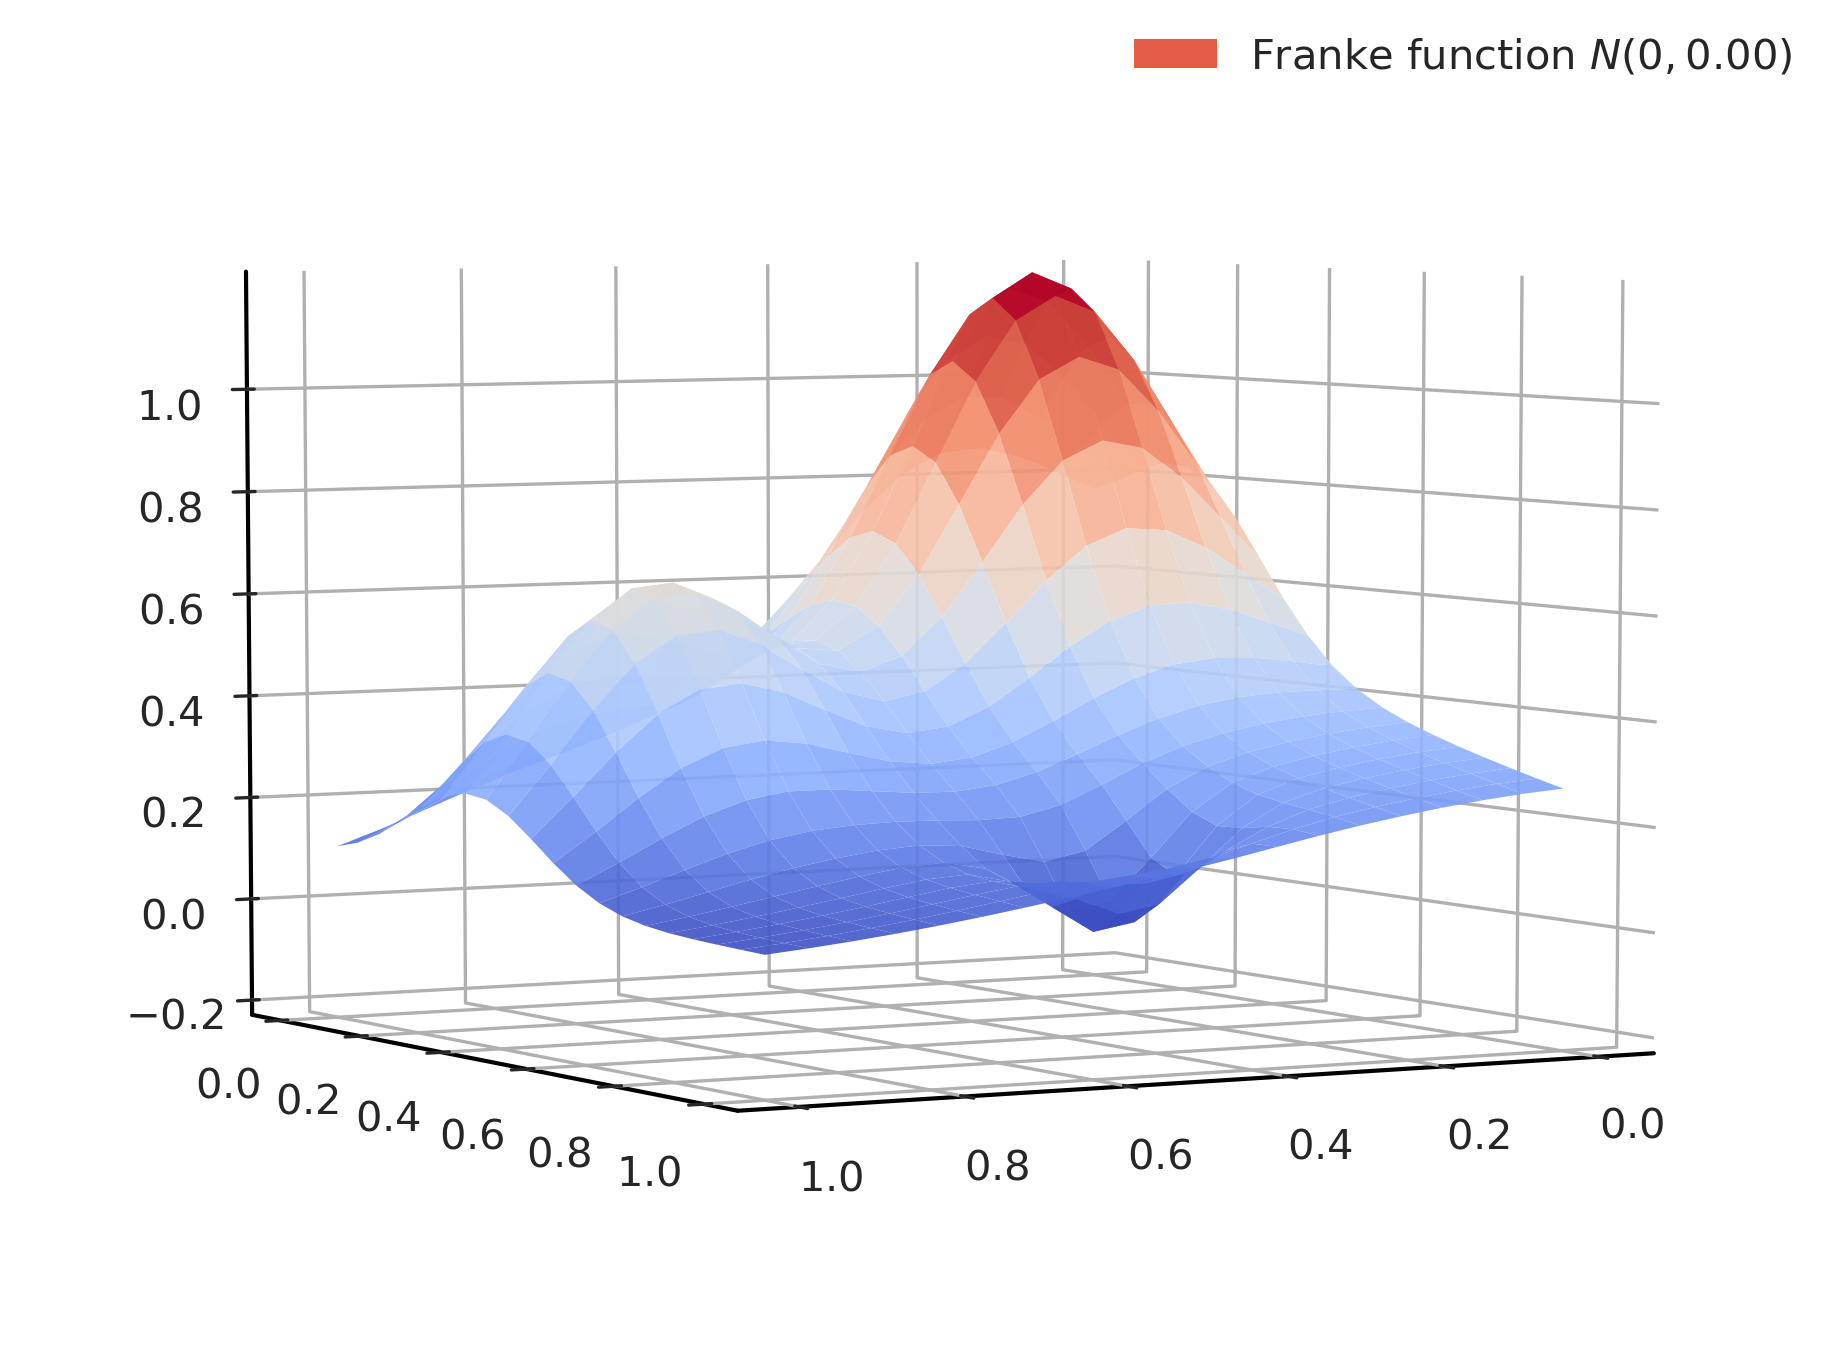
\includegraphics[width=0.45\linewidth]{franke.png}}
\subfloat[$N(0,0.05)$]{\includegraphics[width=0.45\linewidth]{{OLS_L0_P5_franke_N0.05}.png}} \\[-10pt]
\subfloat[$N(0,0.1)$]{\includegraphics[width=0.45\linewidth]{{OLS_L0_P5_franke_N0.1}.png}}
\subfloat[No noise]{\includegraphics[width=0.45\linewidth]{{OLS_L0_P5_franke_N0}.png}}
\captionof{figure}{The Franke function surface and OLS Regression applied to it with varying degrees of noise. Even with high noise, OLS does a good job of modelling the Franke function.\label{fig:OLSfranke}}
\end{figure*}

\subsubsection{Ridge regression}
Next, we look at the effect of an additional regularization term on our model fitting procedure. First off, we note that overfitting and high variance only became a problem at very high model complexities, we therefore do not expect a drastic improvement using the test data that we already got with OLS.

First and foremost, we explore the dependence on the shrinkage parameter. As we can see by the model fits in figure \ref{fig:lassofranke}, increasing the $\lambda$, or shrinkage parameter, the model is simplified, as we penalize high values of beta. This can again be seen in figure \ref{fig:lambdasridge}, where the variance of the betas decrease with the shrinkage parameter. Furthermore, our error plot, figure \ref{fig:BVrl}, shows that we no longer get a sharp increase in error for large complexities. However, the overall error is lower using a simple OLS method for this data set, but the ridge method could potentially prove useful in a case where there is danger of over-fitting.


\subsubsection{Lasso regression}
Lastly, we look at Lasso regression. Applying it to the Franke function, we see that its behaviour is very similar to that of Ridge regression, which is expected. Since both methods employ a regularization term to constrain the beta values, we see on the right in figure \ref{fig:lambdasridge} that each beta converge towards zero, but as opposed to Ridge, the Lasso values actually go to true zero. Furthermore, \ref{fig:lassofranke} shows some of the Lasso fits to the Franke function, and how large values of the shrinkage parameter sets all $\beta$-coefficients to zero. Additionally, \ref{fig:BVrl} shows that very low $\lambda$-values, show the best result, and that we don't gain much from increasing the polynomial degree past 5, however, we note that as with Ridge, we no longer fit to noise for large model complexities as we did for OLS.

\subsection{Terrain data}
In this section we apply all our methods to the terrain data. The motivation for applying our model to these data is so that we can properly study the benefits of Ridge and Lasso regression. As we saw in the previous analysis, OLS won out, because we never require high enough polynomial degree so that overfitting becomes a significant problem. However, the terrain data has less predictable slopes and higher noise levels, as can be seen in figure \ref{fig:terrain}.

For this study, we have applied our methods for many different polynomial degrees and $\lambda$ values, only a few of which are presented here.
First, we looked at the error response per $\lambda$ value, which revealed that we have no significant decrease for Ridge nor Lasso past $\lambda=10^{-5}$. The error over polynomial degrees using this value of the shrinkage parameter can be seen in figure \ref{fig:BVterrain}. As we can see, OLS has a positive trend, but breaks down at degrees higher than 8, and is beaten by Ridge regression! Although Lasso never collapses like the other two, it seems to converge on a higher MSE for very high polynomial degrees. The figure suggests that decreasing the $\lambda$ value further could allow for a more complex model fit for Lasso, but this had minimal effect. Another visualization of the behaviour of our models at a polynomial complexity of degree 10 can be seen in figure \ref{fig:terrain}, where we see how OLS decides to party instead.




%% ---------------
%% CONCLUSION
\section{Summary Remarks}
In this project we have looked at three different regression methods, applied to two different types of data. First, we looked at how our methods respond to a nicely behaved Franke function, before we applied it to the jagged and unpredictable behaviour of M\o svatn. We conclude that for the simple Franke case, the OLS comes out as the winner by far. The additions of regularizing terms does not seem to have a major impact even considering very high noise levels. However, when applied to the terrain data, OLS loses to Ridge regression, which is amble to constrain the $\beta$ values to reasonable values for longer. Lasso, however, is too crude and strict on its $\beta$'s, resulting in under-performing predictions and inability to adapt to the real world, depression and insecurity.

\printbibliography

\clearpage
\begin{figure*}[p]
\centering
\subfloat[Ridge regression]{\includegraphics[width=0.45\linewidth]{{BV_ridge_L+0.01_N0.1_franke_N0.1}.png}}
\subfloat[Lasso regression]{\includegraphics[width=0.45\linewidth]{{BV_lasso_L+0.01_N0.1_franke_N0.1}.png}}
\captionof{figure}{MSE error, bias and variance when using Ridge and Lasso regression with different $\lambda$ parameters on the Franke function with Gaussian noise $N(0,0.1)$. Plotted using $\lambda = [ 10^{-6}, 10^{-5}, 10^{-4}, 10^{-3}, 10^{-2}]$ over 15 polynomial degrees. \label{fig:BVrl}}
\end{figure*}

\begin{figure*}[p]
\centering
\subfloat[Ridge $\lambda=0.1$]{\includegraphics[width=0.45\linewidth]{{ridge_L0.1_P5_franke_N0.05}.png}} 
\subfloat[Ridge $\lambda=0.01$]{\includegraphics[width=0.45\linewidth]{{ridge_L0.01_P5_franke_N0.05}.png}}\\[-10pt]
\subfloat[Ridge $\lambda=0.001$]{\includegraphics[width=0.45\linewidth]{{ridge_L0.001_P5_franke_N0.05}.png}}
\subfloat[Ridge $\lambda=0.0001$]{\includegraphics[width=0.45\linewidth]{{ridge_L0.0001_P5_franke_N0.05}.png}}
\captionof{figure}{Ridge Regression for four different values of the $\lambda$ parameter. For this analysis, we obtain the best fits with small values of $\lambda$, which brings us closer to OLS.}
\label{fig:ridgefranke}
\end{figure*}

\clearpage
\begin{figure*}[p]
\centering
\subfloat[Lasso $\lambda=0.1$]{\includegraphics[width=0.45\linewidth]{{lasso_L0.1_P5_franke_N0.05}.png}} 
\subfloat[Lasso $\lambda=0.01$]{\includegraphics[width=0.45\linewidth]{{lasso_L0.01_P5_franke_N0.05}.png}}\\[-10pt]
\subfloat[Lasso $\lambda=0.001$]{\includegraphics[width=0.45\linewidth]{{lasso_L0.001_P5_franke_N0.05}.png}}
\subfloat[Lasso $\lambda=0.0001$]{\includegraphics[width=0.45\linewidth]{{lasso_L0.0001_P5_franke_N0.05}.png}}
\captionof{figure}{Lasso Regression for four values of $\lambda$. Even for small $\lambda$s, the fits are very crude.}
\label{fig:lassofranke}
\end{figure*}


\begin{figure*}[p]
\centering
\subfloat[Ridge regression]{\includegraphics[width=0.45\linewidth]{{ridge_lambdas}.png}}
\subfloat[Ridge regression]{\includegraphics[width=0.45\linewidth]{{lasso_lambdas}.png}}
\captionof{figure}{Values for the 14 first $\beta$-values using a 5th degree polynomial fit for different values of the shrinkage parameter $\lambda$ using Ridge and Lasso regression. Confidence per parameter is calculated across all K-Folds, and plotted as error bars.}
\label{fig:lambdasridge}
\end{figure*}

\clearpage

\begin{figure*}[p]
\centering
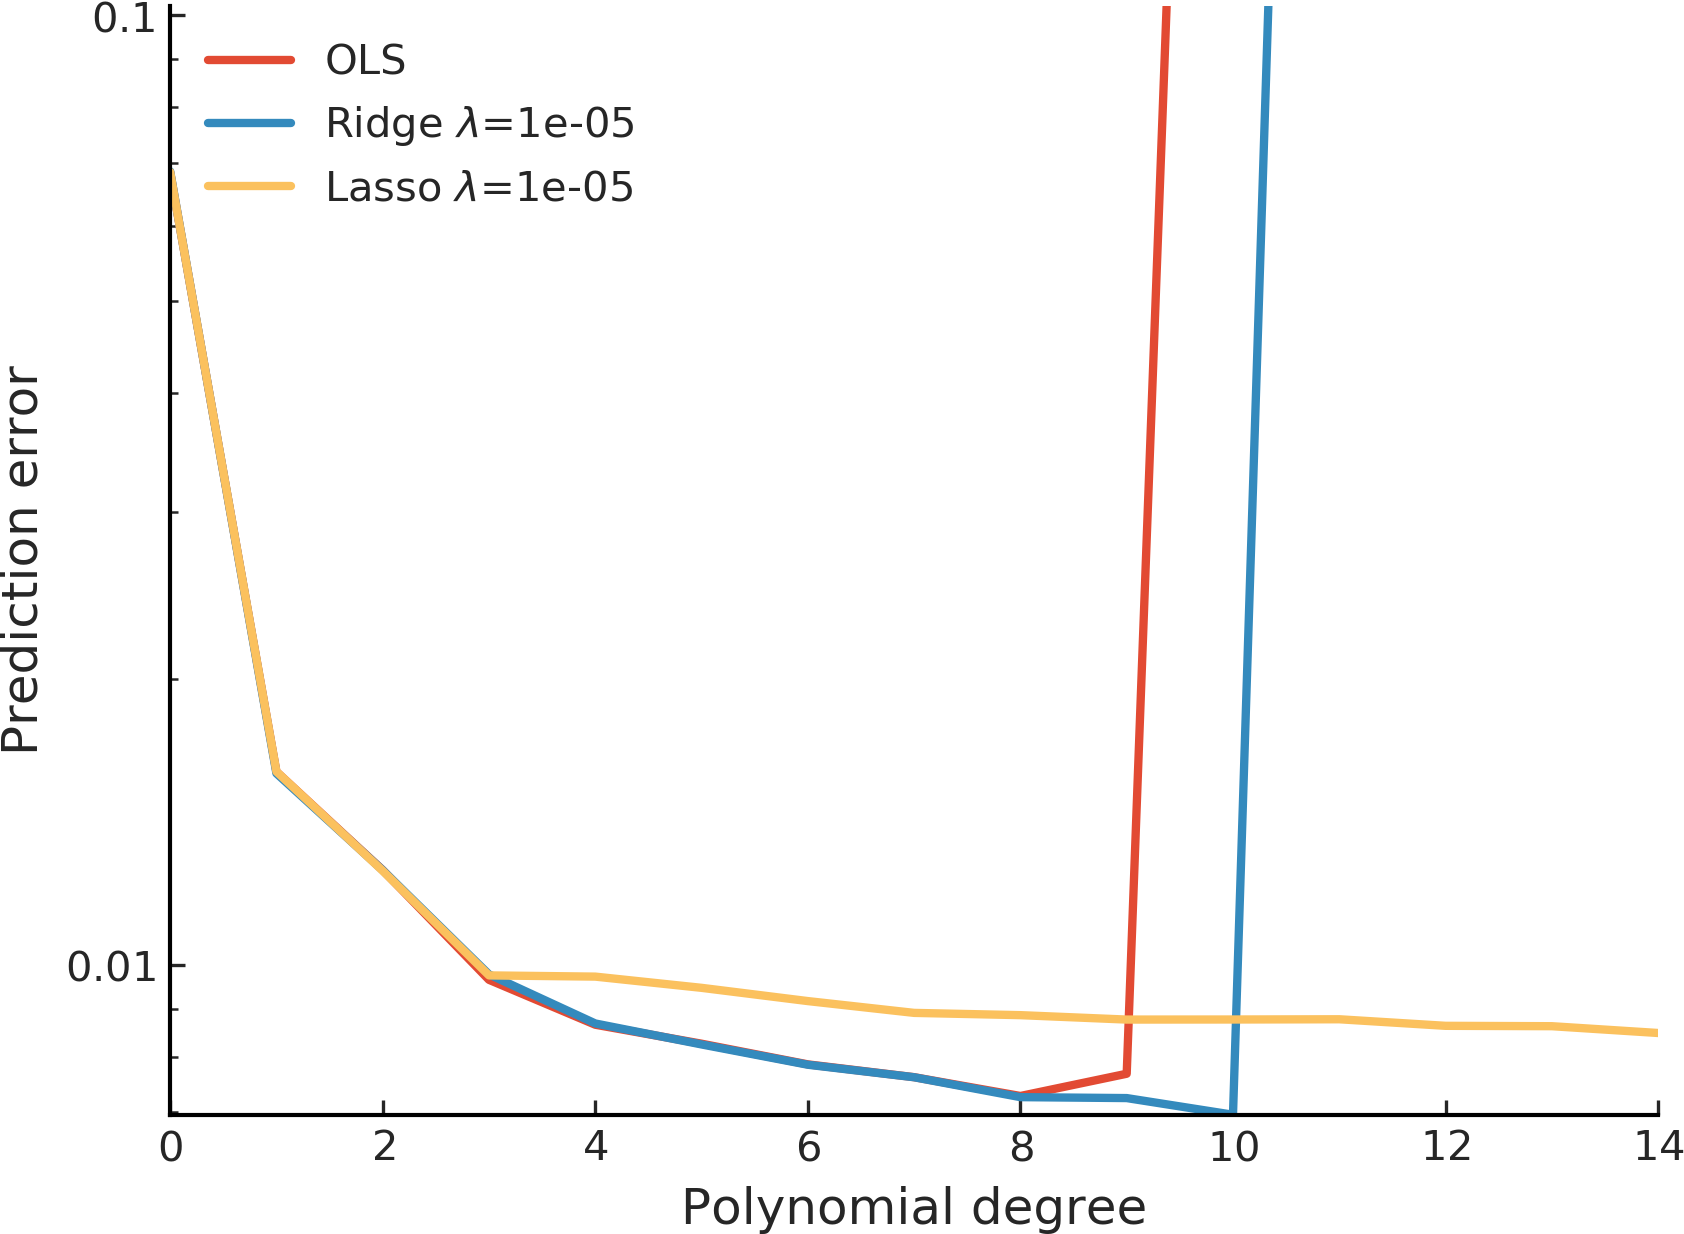
\includegraphics[width=0.4\linewidth]{BV_terrain.png}
\captionof{figure}{The MSE error for the terrain fits. We note how OLS collapses at polynomial degree 8, and is beaten by Ridge regression which carries on to degree 10. Although lasso regression does not collapse in the way Ridge and OLS does, it seems to converge on a higher MSE for very high complexities. \label{fig:BVterrain}}
\end{figure*}

\begin{figure*}[p]
\centering
\subfloat[Terrain data]{\includegraphics[width=0.45\linewidth]{{terrain}.png}}
\subfloat[OLS]{\includegraphics[width=0.45\linewidth]{{OLS_L1e-05_P10_terrain}.png}}\\[-10pt]
\subfloat[Ridge $\lambda=10^{-5}$]{\includegraphics[width=0.45\linewidth]{{ridge_L1e-05_P10_terrain}.png}}
\subfloat[Lasso $\lambda=10^{-5}$]{\includegraphics[width=0.45\linewidth]{{lasso_L1e-05_P10_terrain}.png}}
\captionof{figure}{Polynomial fits on terrain data for a degree 10 polynomial. As we can see, this time, the OLS method collapses above degree 8, while Ridge regression makes a good fit and Lasso struggles to capture the details. \label{fig:terrain}}
\end{figure*}
\clearpage
%\end{multicols}

\end{document}
